% Options for packages loaded elsewhere
\PassOptionsToPackage{unicode}{hyperref}
\PassOptionsToPackage{hyphens}{url}
%
\documentclass[
]{article}
\usepackage{lmodern}
\usepackage{amssymb,amsmath}
\usepackage{ifxetex,ifluatex}
\ifnum 0\ifxetex 1\fi\ifluatex 1\fi=0 % if pdftex
  \usepackage[T1]{fontenc}
  \usepackage[utf8]{inputenc}
  \usepackage{textcomp} % provide euro and other symbols
\else % if luatex or xetex
  \usepackage{unicode-math}
  \defaultfontfeatures{Scale=MatchLowercase}
  \defaultfontfeatures[\rmfamily]{Ligatures=TeX,Scale=1}
\fi
% Use upquote if available, for straight quotes in verbatim environments
\IfFileExists{upquote.sty}{\usepackage{upquote}}{}
\IfFileExists{microtype.sty}{% use microtype if available
  \usepackage[]{microtype}
  \UseMicrotypeSet[protrusion]{basicmath} % disable protrusion for tt fonts
}{}
\makeatletter
\@ifundefined{KOMAClassName}{% if non-KOMA class
  \IfFileExists{parskip.sty}{%
    \usepackage{parskip}
  }{% else
    \setlength{\parindent}{0pt}
    \setlength{\parskip}{6pt plus 2pt minus 1pt}}
}{% if KOMA class
  \KOMAoptions{parskip=half}}
\makeatother
\usepackage{xcolor}
\IfFileExists{xurl.sty}{\usepackage{xurl}}{} % add URL line breaks if available
\IfFileExists{bookmark.sty}{\usepackage{bookmark}}{\usepackage{hyperref}}
\hypersetup{
  pdftitle={Central Limit Theorem},
  hidelinks,
  pdfcreator={LaTeX via pandoc}}
\urlstyle{same} % disable monospaced font for URLs
\usepackage[margin=1in]{geometry}
\usepackage{color}
\usepackage{fancyvrb}
\newcommand{\VerbBar}{|}
\newcommand{\VERB}{\Verb[commandchars=\\\{\}]}
\DefineVerbatimEnvironment{Highlighting}{Verbatim}{commandchars=\\\{\}}
% Add ',fontsize=\small' for more characters per line
\usepackage{framed}
\definecolor{shadecolor}{RGB}{248,248,248}
\newenvironment{Shaded}{\begin{snugshade}}{\end{snugshade}}
\newcommand{\AlertTok}[1]{\textcolor[rgb]{0.94,0.16,0.16}{#1}}
\newcommand{\AnnotationTok}[1]{\textcolor[rgb]{0.56,0.35,0.01}{\textbf{\textit{#1}}}}
\newcommand{\AttributeTok}[1]{\textcolor[rgb]{0.77,0.63,0.00}{#1}}
\newcommand{\BaseNTok}[1]{\textcolor[rgb]{0.00,0.00,0.81}{#1}}
\newcommand{\BuiltInTok}[1]{#1}
\newcommand{\CharTok}[1]{\textcolor[rgb]{0.31,0.60,0.02}{#1}}
\newcommand{\CommentTok}[1]{\textcolor[rgb]{0.56,0.35,0.01}{\textit{#1}}}
\newcommand{\CommentVarTok}[1]{\textcolor[rgb]{0.56,0.35,0.01}{\textbf{\textit{#1}}}}
\newcommand{\ConstantTok}[1]{\textcolor[rgb]{0.00,0.00,0.00}{#1}}
\newcommand{\ControlFlowTok}[1]{\textcolor[rgb]{0.13,0.29,0.53}{\textbf{#1}}}
\newcommand{\DataTypeTok}[1]{\textcolor[rgb]{0.13,0.29,0.53}{#1}}
\newcommand{\DecValTok}[1]{\textcolor[rgb]{0.00,0.00,0.81}{#1}}
\newcommand{\DocumentationTok}[1]{\textcolor[rgb]{0.56,0.35,0.01}{\textbf{\textit{#1}}}}
\newcommand{\ErrorTok}[1]{\textcolor[rgb]{0.64,0.00,0.00}{\textbf{#1}}}
\newcommand{\ExtensionTok}[1]{#1}
\newcommand{\FloatTok}[1]{\textcolor[rgb]{0.00,0.00,0.81}{#1}}
\newcommand{\FunctionTok}[1]{\textcolor[rgb]{0.00,0.00,0.00}{#1}}
\newcommand{\ImportTok}[1]{#1}
\newcommand{\InformationTok}[1]{\textcolor[rgb]{0.56,0.35,0.01}{\textbf{\textit{#1}}}}
\newcommand{\KeywordTok}[1]{\textcolor[rgb]{0.13,0.29,0.53}{\textbf{#1}}}
\newcommand{\NormalTok}[1]{#1}
\newcommand{\OperatorTok}[1]{\textcolor[rgb]{0.81,0.36,0.00}{\textbf{#1}}}
\newcommand{\OtherTok}[1]{\textcolor[rgb]{0.56,0.35,0.01}{#1}}
\newcommand{\PreprocessorTok}[1]{\textcolor[rgb]{0.56,0.35,0.01}{\textit{#1}}}
\newcommand{\RegionMarkerTok}[1]{#1}
\newcommand{\SpecialCharTok}[1]{\textcolor[rgb]{0.00,0.00,0.00}{#1}}
\newcommand{\SpecialStringTok}[1]{\textcolor[rgb]{0.31,0.60,0.02}{#1}}
\newcommand{\StringTok}[1]{\textcolor[rgb]{0.31,0.60,0.02}{#1}}
\newcommand{\VariableTok}[1]{\textcolor[rgb]{0.00,0.00,0.00}{#1}}
\newcommand{\VerbatimStringTok}[1]{\textcolor[rgb]{0.31,0.60,0.02}{#1}}
\newcommand{\WarningTok}[1]{\textcolor[rgb]{0.56,0.35,0.01}{\textbf{\textit{#1}}}}
\usepackage{graphicx,grffile}
\makeatletter
\def\maxwidth{\ifdim\Gin@nat@width>\linewidth\linewidth\else\Gin@nat@width\fi}
\def\maxheight{\ifdim\Gin@nat@height>\textheight\textheight\else\Gin@nat@height\fi}
\makeatother
% Scale images if necessary, so that they will not overflow the page
% margins by default, and it is still possible to overwrite the defaults
% using explicit options in \includegraphics[width, height, ...]{}
\setkeys{Gin}{width=\maxwidth,height=\maxheight,keepaspectratio}
% Set default figure placement to htbp
\makeatletter
\def\fps@figure{htbp}
\makeatother
\setlength{\emergencystretch}{3em} % prevent overfull lines
\providecommand{\tightlist}{%
  \setlength{\itemsep}{0pt}\setlength{\parskip}{0pt}}
\setcounter{secnumdepth}{-\maxdimen} % remove section numbering

\title{Central Limit Theorem}
\author{}
\date{\vspace{-2.5em}}

\begin{document}
\maketitle

\hypertarget{exploration-of-the-central-limit-theorem}{%
\section{Exploration of the Central Limit
Theorem}\label{exploration-of-the-central-limit-theorem}}

\hypertarget{the-central-limit-thereom-is-one-of-the-most-fundamental-concepts-in-statistics.-in-this-document-i-will-be-visualizing-the-central-limit-theorem-to-better-drive-my-understand-of-this-concept.-the-theorem-itself-revolves-around-the-sampling-process-in-which-we-try-to-approximate-the-distribution-of-the-population-by-drawing-values-from-the-whole-population.-the-underlying-assumption-that-we-cannot-sample-the-whole-population-so-we-sample-until-we-feel-that-we-have-an-accurate-estimation-of-our-population.}{%
\subsection{The Central Limit Thereom is one of the most fundamental
concepts in statistics. In this document, I will be visualizing the
central limit theorem to better drive my understand of this concept. The
theorem itself revolves around the sampling process, in which we try to
approximate the distribution of the population by drawing values from
the whole population. The underlying assumption that we cannot sample
the whole population, so we sample until we feel that we have an
accurate estimation of our
population.}\label{the-central-limit-thereom-is-one-of-the-most-fundamental-concepts-in-statistics.-in-this-document-i-will-be-visualizing-the-central-limit-theorem-to-better-drive-my-understand-of-this-concept.-the-theorem-itself-revolves-around-the-sampling-process-in-which-we-try-to-approximate-the-distribution-of-the-population-by-drawing-values-from-the-whole-population.-the-underlying-assumption-that-we-cannot-sample-the-whole-population-so-we-sample-until-we-feel-that-we-have-an-accurate-estimation-of-our-population.}}

\hypertarget{for-this-example-we-will-assume-our-population-is-100000-males-that-live-in-a-hypothetical-country.-we-can-say-that-the-height-of-all-the-males-ranges-from-1.5-m-4.9-feet-to-2-m-6.6-feet.-our-population-follows-the-following-distribution-mean-is-shown-by-a-vertical-red-line}{%
\subsubsection{For this example, we will assume our population is
100,000 males that live in a hypothetical country. We can say that the
height of all the males ranges from 1.5 m (\textasciitilde4.9 feet) to 2
m (\textasciitilde6.6 feet). Our population follows the following
distribution (mean is shown by a vertical red
line):}\label{for-this-example-we-will-assume-our-population-is-100000-males-that-live-in-a-hypothetical-country.-we-can-say-that-the-height-of-all-the-males-ranges-from-1.5-m-4.9-feet-to-2-m-6.6-feet.-our-population-follows-the-following-distribution-mean-is-shown-by-a-vertical-red-line}}

\begin{Shaded}
\begin{Highlighting}[]
\NormalTok{height_dist <-}\StringTok{ }\KeywordTok{runif}\NormalTok{(}\DecValTok{100000}\NormalTok{, }\FloatTok{1.5}\NormalTok{, }\DecValTok{2}\NormalTok{)}
\NormalTok{mean_height <-}\StringTok{ }\KeywordTok{mean}\NormalTok{(height_dist)}
\KeywordTok{hist}\NormalTok{(height_dist, }
     \DataTypeTok{main =} \StringTok{'Height Distribution for 100,000 Males'}\NormalTok{,}
     \DataTypeTok{xlab =} \StringTok{'Height in M'}\NormalTok{,}
     \DataTypeTok{breaks =} \DecValTok{100}\NormalTok{)}
\KeywordTok{abline}\NormalTok{(}\DataTypeTok{v=}\NormalTok{mean_height,}\DataTypeTok{col=}\StringTok{"red"}\NormalTok{)}
\end{Highlighting}
\end{Shaded}

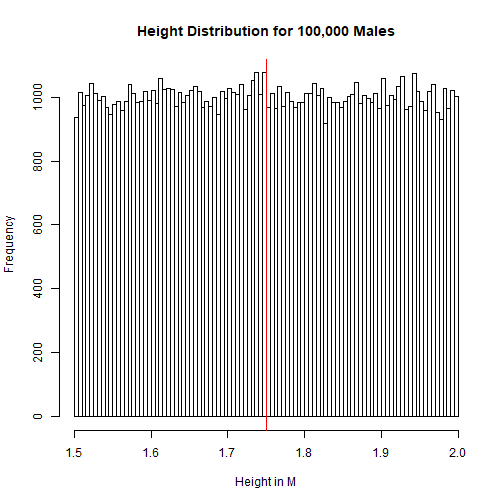
\includegraphics{clt_files/figure-latex/unnamed-chunk-1-1.pdf}

\hypertarget{given-this-population-we-hope-to-run-an-experiment-to-try-and-approximate-this-distribution.-since-we-cant-sample-all-100000-males-we-decide-our-best-course-of-action-is-to-complete-simple-random-sampling-srs.-below-is-a-function-to-create-samples-with-size-n-for-reps-repetitions-from-a-distribution-dist}{%
\subsubsection{Given this population, we hope to run an experiment to
try and approximate this distribution. Since we ``can't'' sample all
100000 males, we decide our best course of action is to complete simple
random sampling (SRS). Below is a function to create samples with size N
for reps repetitions from a distribution
dist:}\label{given-this-population-we-hope-to-run-an-experiment-to-try-and-approximate-this-distribution.-since-we-cant-sample-all-100000-males-we-decide-our-best-course-of-action-is-to-complete-simple-random-sampling-srs.-below-is-a-function-to-create-samples-with-size-n-for-reps-repetitions-from-a-distribution-dist}}

\begin{Shaded}
\begin{Highlighting}[]
\CommentTok{# Function takes the sample size N, the number of sampling repetitions to complete and distribution to sample from}

\NormalTok{sampl <-}\StringTok{ }\ControlFlowTok{function}\NormalTok{(n, reps, dist) \{}
\NormalTok{  samples <-}\StringTok{ }\KeywordTok{replicate}\NormalTok{(reps, }\KeywordTok{sample}\NormalTok{(dist, n))}
\NormalTok{  sample_means <-}\StringTok{ }\KeywordTok{colMeans}\NormalTok{(samples)}
  \KeywordTok{return}\NormalTok{(sample_means)}
\NormalTok{\}}
\end{Highlighting}
\end{Shaded}

\hypertarget{lets-start-with-samples-of-size-3-for-100-repetitions-from-our-testing-distribution}{%
\subsubsection{Lets start with samples of size 3 for 100 repetitions
from our testing
distribution:}\label{lets-start-with-samples-of-size-3-for-100-repetitions-from-our-testing-distribution}}

\begin{Shaded}
\begin{Highlighting}[]
\NormalTok{means <-}\StringTok{ }\KeywordTok{sampl}\NormalTok{(}\DecValTok{3}\NormalTok{, }\DecValTok{1000}\NormalTok{, height_dist)}
\KeywordTok{hist}\NormalTok{(means)}
\end{Highlighting}
\end{Shaded}

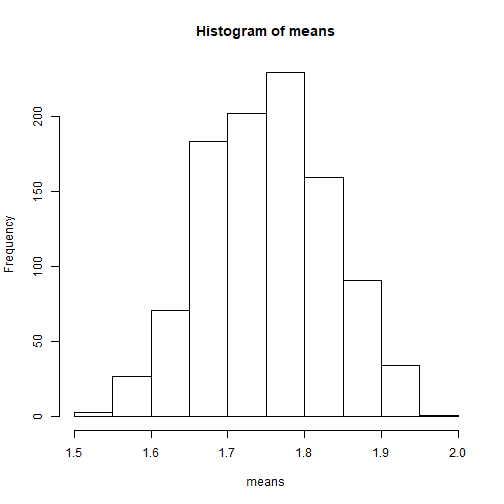
\includegraphics{clt_files/figure-latex/unnamed-chunk-3-1.pdf}

\hypertarget{this-is-where-the-central-limit-theorem-comes-into-play-as-we-increase-our-sample-size-n-the-resulting-sampling-distribution-the-distribution-of-our-sample-means-will-begin-to-resemble-the-normal-distribution}{%
\subsubsection{This is where the central limit theorem comes into play:
as we increase our sample size (N), the resulting sampling distribution
(the distribution of our sample means) will begin to resemble the normal
distribution:}\label{this-is-where-the-central-limit-theorem-comes-into-play-as-we-increase-our-sample-size-n-the-resulting-sampling-distribution-the-distribution-of-our-sample-means-will-begin-to-resemble-the-normal-distribution}}

\begin{Shaded}
\begin{Highlighting}[]
\KeywordTok{hist}\NormalTok{(}\KeywordTok{sampl}\NormalTok{(}\DecValTok{10}\NormalTok{, }\DecValTok{1000}\NormalTok{, height_dist))}
\end{Highlighting}
\end{Shaded}

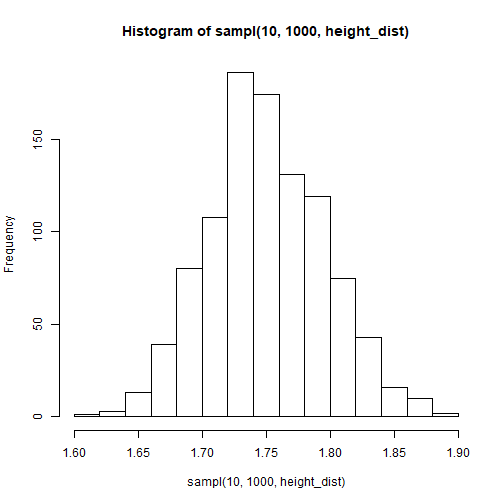
\includegraphics{clt_files/figure-latex/unnamed-chunk-4-1.pdf}

\begin{Shaded}
\begin{Highlighting}[]
\KeywordTok{hist}\NormalTok{(}\KeywordTok{sampl}\NormalTok{(}\DecValTok{20}\NormalTok{, }\DecValTok{1000}\NormalTok{, height_dist))}
\end{Highlighting}
\end{Shaded}

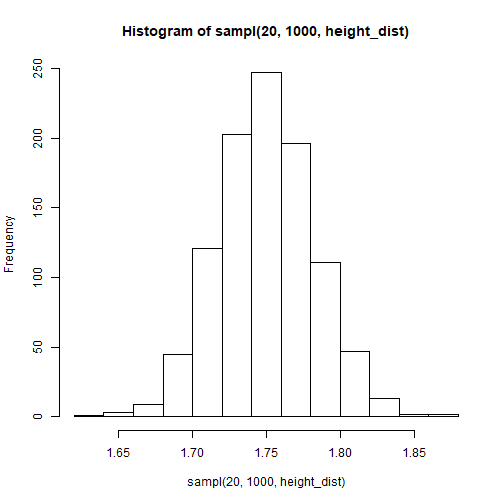
\includegraphics{clt_files/figure-latex/unnamed-chunk-5-1.pdf}

\begin{Shaded}
\begin{Highlighting}[]
\KeywordTok{hist}\NormalTok{(}\KeywordTok{sampl}\NormalTok{(}\DecValTok{50}\NormalTok{, }\DecValTok{1000}\NormalTok{, height_dist))}
\end{Highlighting}
\end{Shaded}

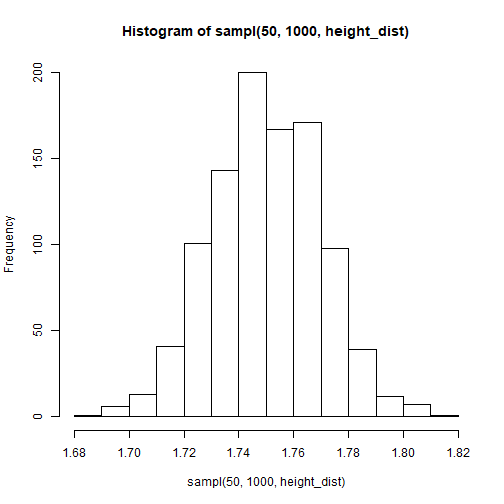
\includegraphics{clt_files/figure-latex/unnamed-chunk-6-1.pdf}

\hypertarget{through-the-proggression-of-the-above-distributions-we-can-see-that-by-only-changing-the-sample-size-n-we-have-approximated-a-normal-distribution}{%
\subsubsection{Through the proggression of the above distributions, we
can see that by only changing the sample size N, we have approximated a
normal
distribution}\label{through-the-proggression-of-the-above-distributions-we-can-see-that-by-only-changing-the-sample-size-n-we-have-approximated-a-normal-distribution}}

\end{document}
